%%%%% this line is 80 chars wide, please don't make longer lines %%%%%%%%%%%%%%%
 This introduction is based on the book "Auditory Neuroscience" 
\cite{AuditoryNeuroscience}, chapter two.

The peripheral auditory system has (generally air) pressure as input, 
and spike trains as output. We will go through the parts of the ear, with help 
of \autoref{fig:ear}.

Let us first consider the external ear. There the pressure signals enters through
 the ear canal and make the eardrum vibrate. 
This takes to the medium ear, through which 
the vibration is propagated by three ossicles : malleus, incus 
and stapes. The farthest part from the external ear of the stapes touches the 
boundary of the cochlea, on the oval window, in the inner ear, 
and causes vibration in its contained liquid. 
The cochlea forms an interface between this mechanical vibration 
and the neural signal of the auditory nerve 
(VII nerve on \autoref{fig:ear}).

%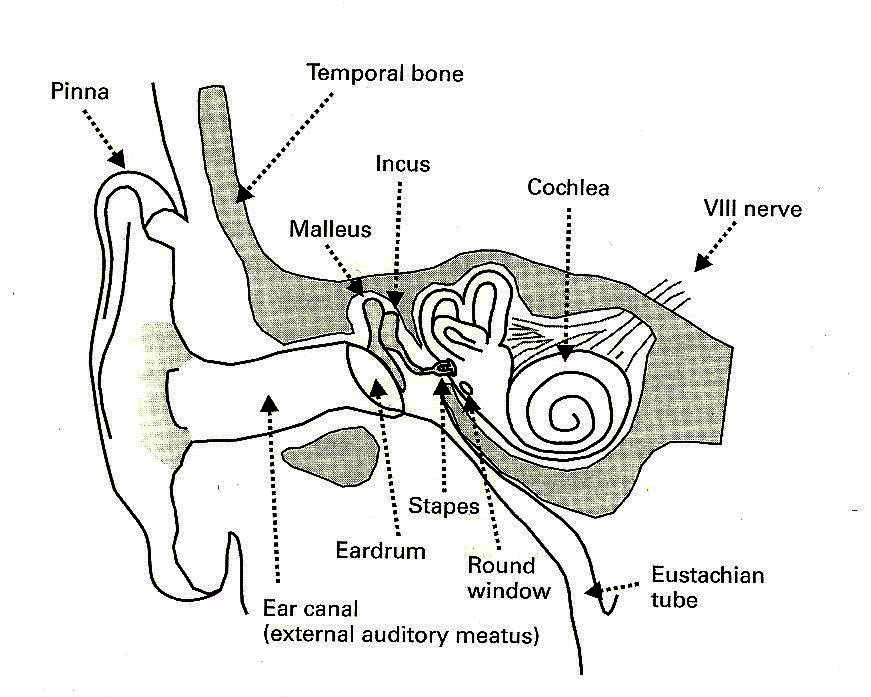
\includegraphics[width=0.45\textwidth]{images/ear-aud52-level.jpg}

\begin{figure}[h]
	\centering
	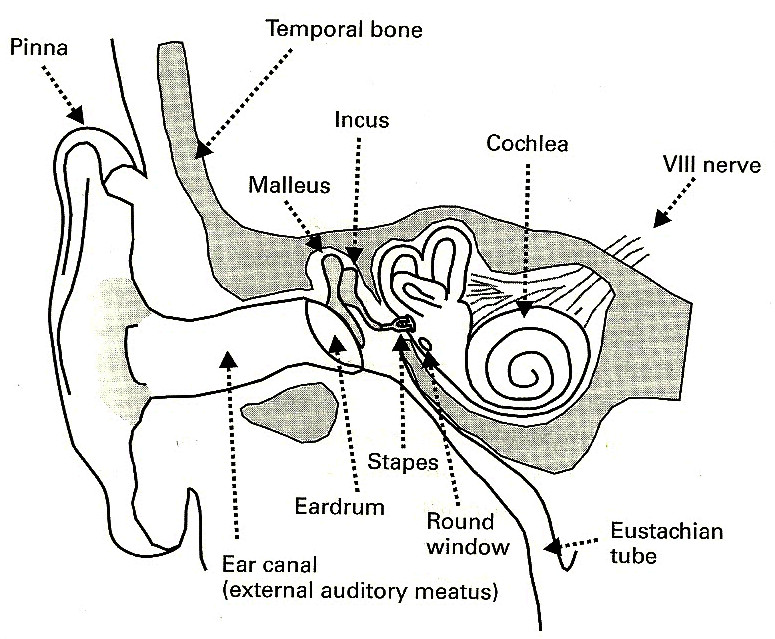
\includegraphics[width=0.45\textwidth]{images/ear2-aud52-level.jpg}
	\caption{Peripheral auditory system (\cite{AuditoryNeuroscience} p.52 )}
	\label{fig:ear}
\end{figure}

%put that one page before the page it should appear on :
%http://www.andrewjpage.com/?archives/48-Figure-spanning-2-columns-in-Latex.html
\begin{figure*}[ht]
	\centering
  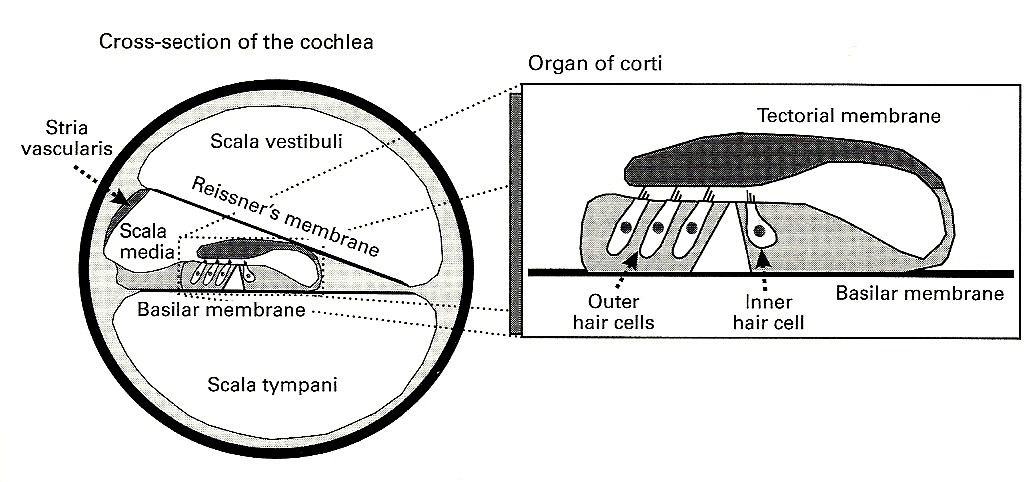
\includegraphics[width=0.75\textwidth]{images/corti2-aud65-level.jpg}
	\caption{Organ of Corti (\cite{AuditoryNeuroscience} p.65 )}
	\label{fig:corti}
\end{figure*}

We will speak more about this interface below. But first we take a closer 
look at the vibration of the cochlea. 
The cochlea is a tube that has two main compartments which are placed on top of 
each other. 
These compartents are separated throughout the cochlear tube by  
the basilar membrane, except at the far end of it where they are joined, 
as can be seen on \autoref{fig:ucochlea}.

%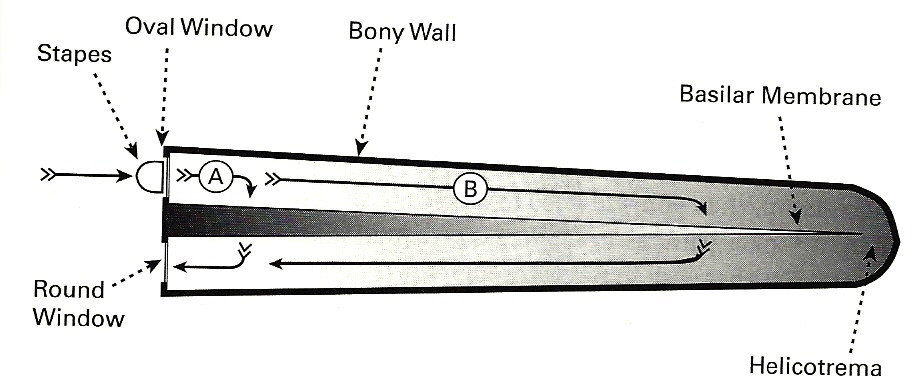
\includegraphics[width=0.45\textwidth]{images/cochlea-aud55-level.jpg}

\begin{figure}[h]
	\centering
	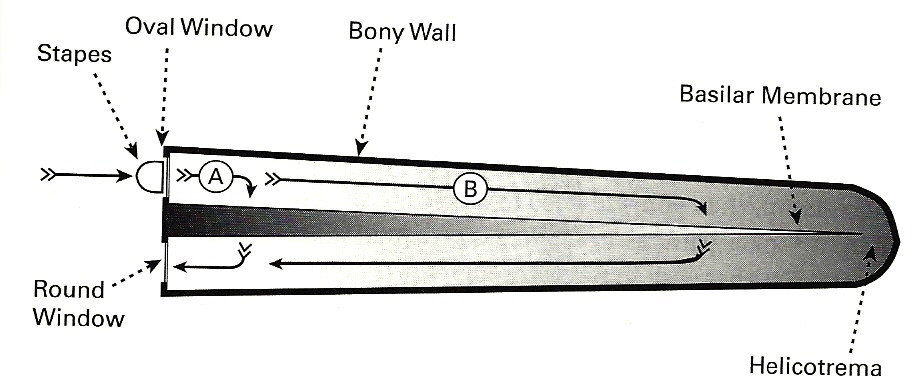
\includegraphics[width=0.45\textwidth]{images/cochlea-aud55-level.jpg}
	\caption{Unrolled cochlea (\cite{AuditoryNeuroscience} p.55 )}
	\label{fig:ucochlea}
\end{figure}


An incoming vibration will propagate through the basilar membrane from 
the upper compartment to the lower. In this process, it will not make all 
the parts of the basilar membrane vibrate at the same intensity. 
In fact, the cochlea is like a "biological Fourier analyzer", in the words of the book.
The frequency content of vibrations is decomposed and each frequency has its 
"favorite" place in the cochlear coiled tube that it makes vibrate particularily. 
The part of the basilar membrane that is the first to vibrate, 
when we gradually put on the volume of a pure tone of frequency f, is said to be of 
"characteristic frequency" f. Near the oval window, the characteristic 
frequencies are high, and as we advance to the tip of the tube, 
the characteristic frequency decreases.

Throughout the cochlear tube spans the organ of Corti, which is the interface
which was previously refered to above in the text. 
We will use \autoref{fig:corti} to illustrate its purpose.

%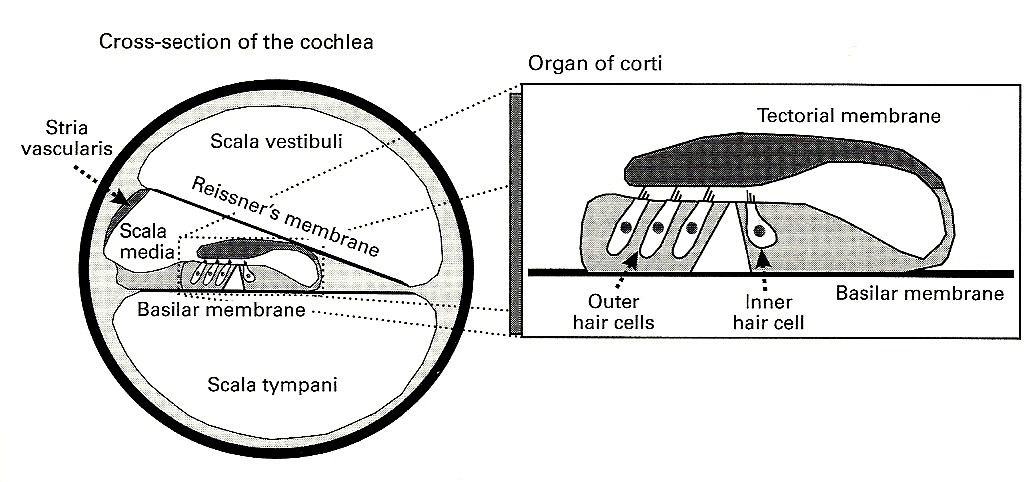
\includegraphics[width=0.45\textwidth]{images/corti2-aud65-level.jpg} %put before, so that then it is at right place

\begin{figure}[h]
	\centering
  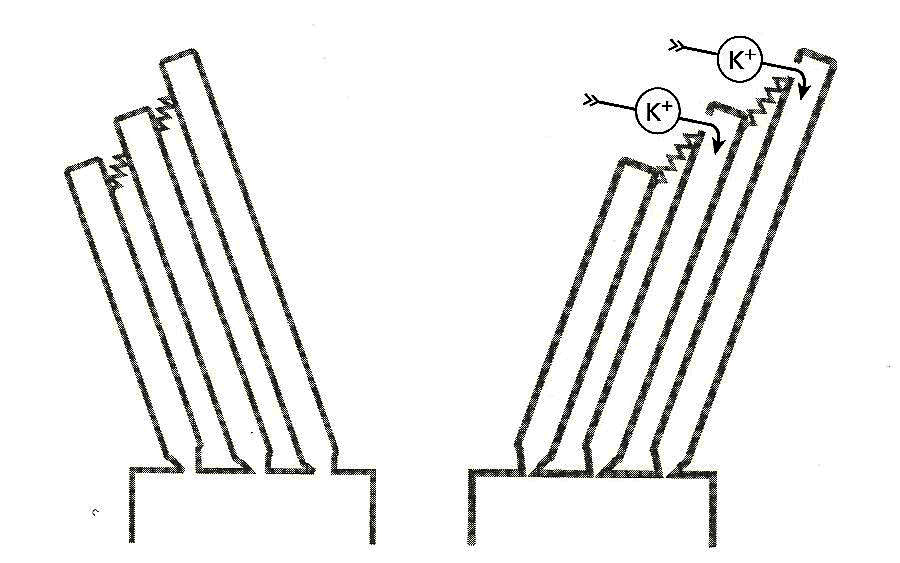
\includegraphics[width=0.45\textwidth]{images/hctransd-aud66-level.jpg}
	\caption{Transduction (\cite{AuditoryNeuroscience} p.66 )}
	\label{fig:transd}
\end{figure}

%model schema
\begin{figure*}[ht]
	\centering
  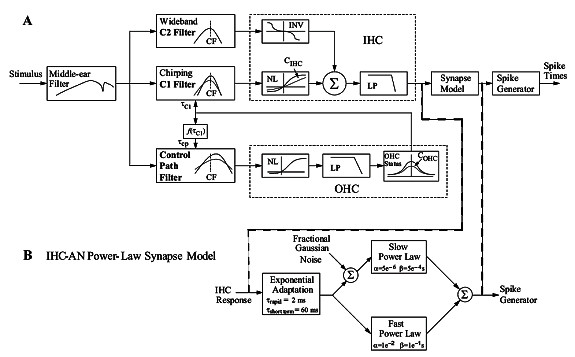
\includegraphics[width=0.75\textwidth]{images/www-bme-rochester-edu-schematicDiagram-level.jpg}
	\caption{Schema of the model (\cite{Model1} their fig. 2). 
	The spike generator (pointed to by an arrow) is 
	the part where the modifications of the model were done}
	\label{fig:modelsch}
\end{figure*}

The upper compartment of the cochlea is in fact in two parts separated by a membrane.
The scala media, where we find the organ of Corti, has a higher 
concentration of potassium cations. A consequence, then is a polarization between
the liquid of the scala media and the inner hair cells. 
When the basilar membrane vibrates, the tectorial membrane does 
that also, and that makes the liquid move. 
These movements cause the deflection of the stereocili 
of the inner hair cells, and when this happens, some potassium ions of the 
scala media go into the inner hair cells (IHC), where they lead to a depolarization.
%The outer hair cells undergo the same process, but , for their part, have a role of amplificator for the liquid movements. %% word about ohc ?
This is depicted in \autoref{fig:transd}.
This depolarization causes glutamate to be released at the synapses %glutamate checked : p75
between the IHC and the auditory nerve fibers, what excites these fibers 
and make them emit action potentials (spikes).

%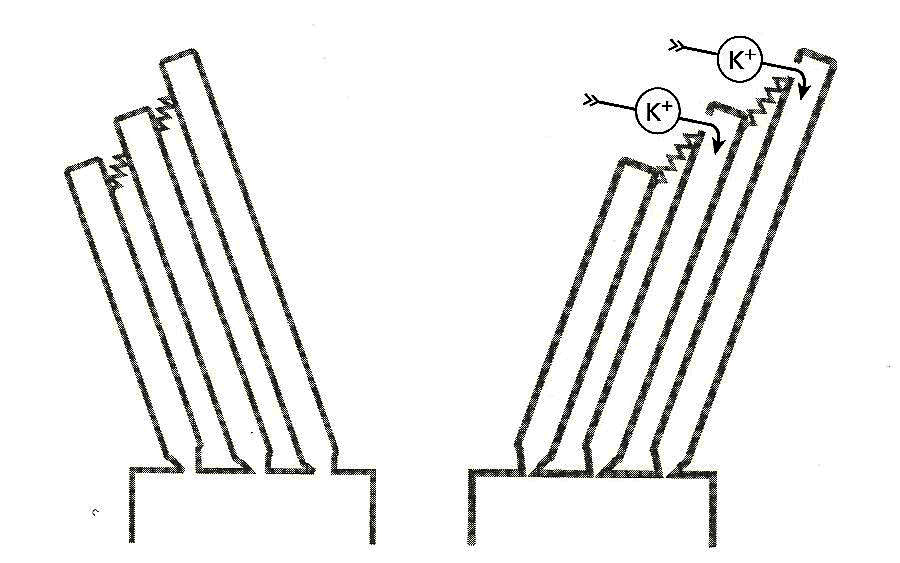
\includegraphics[width=0.45\textwidth]{images/hctransd-aud66-level.jpg}%put before, so that then it is at right place



